\documentclass[unicode,11pt,a4paper,oneside,numbers=endperiod,openany]{scrartcl}

\usepackage{assignment}
\usepackage{textcomp}
\usepackage{graphicx} 
\usepackage{auto-pst-pdf}
\usepackage{float}

\begin{document}

\setassignment
\setduedate{15 October 2019, 13:30}

\serieheader{High Performance Computing}{2019}{Student: Gabriel Fernandes de Oliveira}{Discussed with: N/A}{Solution for Assignment 2}{}
\newline

In this exercise you will practice in data access optimization and performance-oriented programming for cluster environments.


\section{Explaning memory hierarchies \punkte{30}}

    \begin{enumerate}
        \item  The following data was found using the likwid module and the meminfo file, as suggested by the exercise.\\
            \begin{tabular}{| l || c |}
                \hline
                Main memory & 65.69 GB \\ 
                \hline
                L3 cache & 20 MB \\
                \hline
                L2 cache & 256 kB \\
                \hline 
                L1 cache & 32 kB \\
                \hline
            \end{tabular}
        \item  Both graphs were created and added to this assignment: 

        \begin{figure}[H]
            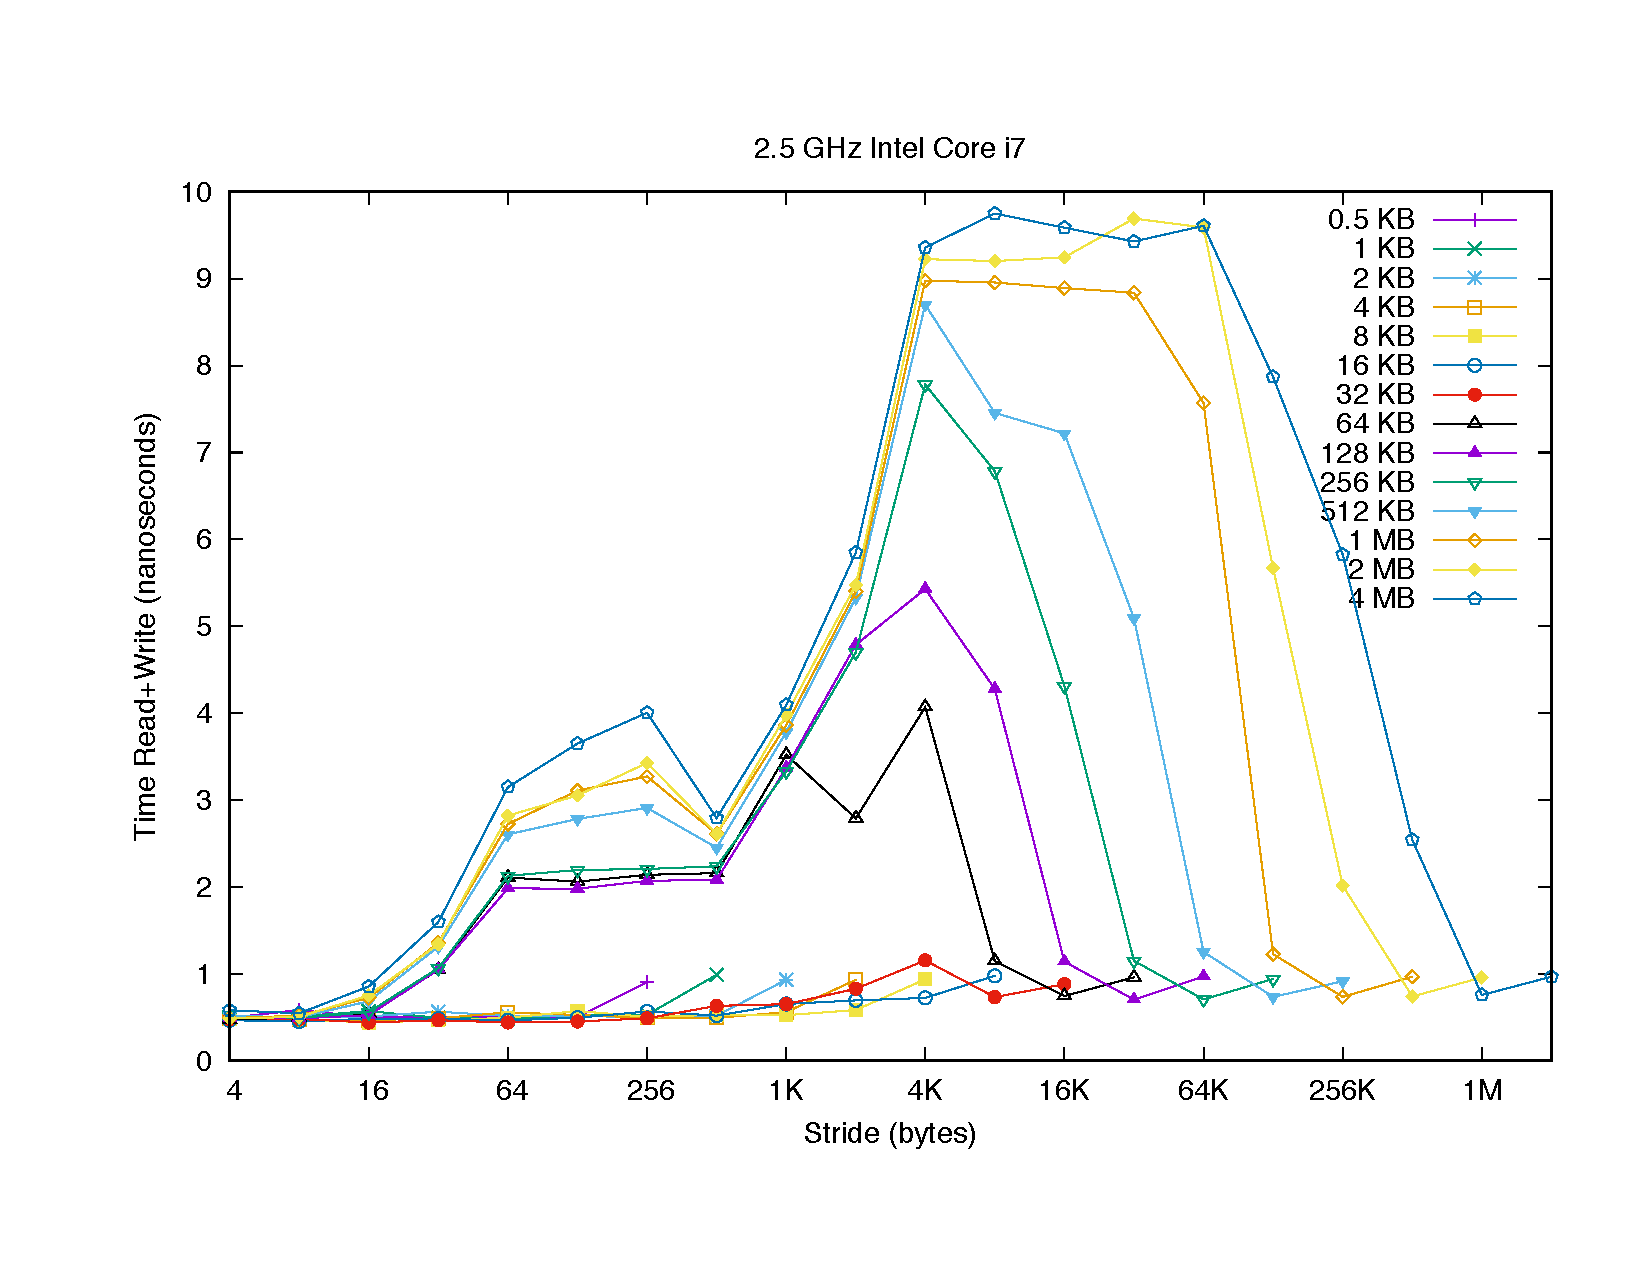
\includegraphics[width=\linewidth]{./membench/generic_mac.pdf}
            \caption{This is the graph generated for my Macbook Pro running on macOS Sierra 10.12.6}
        \end{figure}
        \begin{figure}[H]
            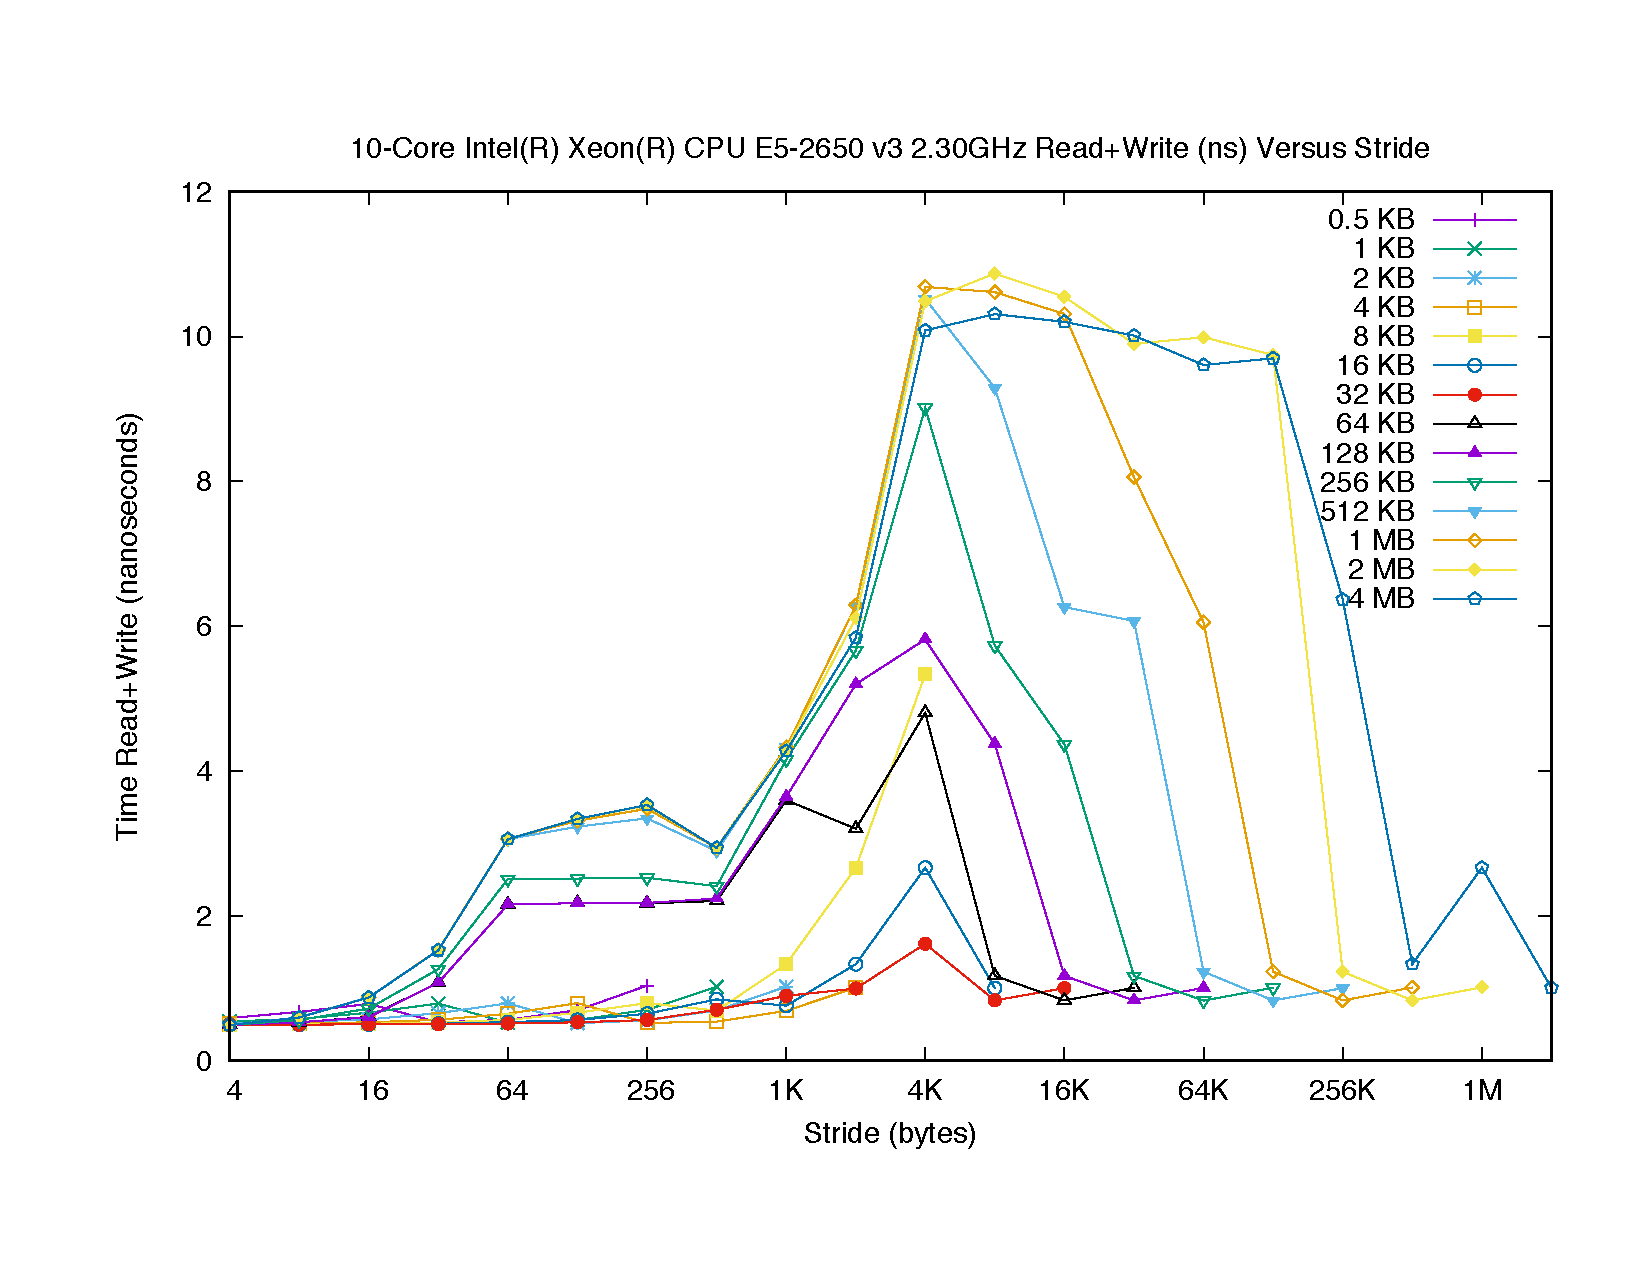
\includegraphics[width=\linewidth]{./membench/generic_icsmaster.pdf}
            \caption{Graph generated on icsmaster}
        \end{figure}
           
        The ps files were also added to this assignment folder, they are called respectivelly generic\_mac.ps and generic\_icsmaster.ps.


        On both graphs the difference between cache response times is very visible.
        The arrays with size $\leq 32kB$ have a very good performance (operations taking around 0.5ns) for every value of stride, since they can be completely stored in L1 cache.
        The arrays with size $\leq 256kB$ show a regular plateau between stride of $64$ and $512$ bytes where read and write takes about 2ns, this is mainly due to the fact that these arrays can be stored in L2 cache, providing a access to the array elements that is slower than that of L1, but is still efficient.
        Finally, another plateau can be noticed for array sizes between $1MB$ and $4MB$, for stride between $4kB$ and $128kB$, this is due to the cache L3, which has a retrieval time worse than that of caches L1 and L2, but still way faster than that of the main memory.

        \item 
            \begin{itemize}
                \item $csize = 128 = 0.5kB$ and $stride = 1 = 4B$
                    This example has a very good performance, around 0.5ns for both icsmaster and my computer, that is mainly due to the good spatial locality associated with a small value of stride.
                    Because the stride is $1$, every element loaded in a cache line will be used, hence the good spatial locality and performance of this case.

                \item $csize = 2^{20} = 4MB$ and $stride = csize/2 = 2^{19} = 2MB$
                    This is another extreme case with a good performance, the read+write takes about 1ns for both computers, that is due to the temporal locality associated with traversing the same elements already loaded on cache.
                    
                    Since the stride is half the size of the array only two elements of the array are being accessed every time the array is traversed.
                    On the first array traversal these two elements are loaded into the cache, and on all following traversals they are retrieved directly from cache, hence the good temporal locality and performance also visible in this case.
            \end{itemize}

        \item  The points with best temporal locality in the graph are the ones closes to the end of each line.
            For example, for the array of size $4MB$, the stride values $2MB$ and $1MB$ offer a very good temporal locality.
            This happens because with a large stride value, few elements of the array are accessed. 
            These few elements accessed can all fit into the cache, and are reused many times since the array is being traversed multiple times, hence the good temporal locality and the high performance on these conditions.

            One can notice similar high performances on other array sizes, when the stride value is close to half or a quarter of the array size.

            Another example of good temporal locality happens for small array sizes ($\leq 32KB$), since these arrays can be fully stored on the L1 cache.
            The first time that the array is traversed every element is loaded into the cache, then for every following traversal the whole array is on cache, so the cache elements are simply reused.

    \end{enumerate}

    \section{Optimize Square Matrix-Matrix Multiplication  \punkte{70}}

    \begin{enumerate}
        \item My implementation of the block matrix multiplication (figure \ref{code}) follows the one provided in pseudo-code in the motivation file as seen in figure \ref{pseudocode}:
            \begin{figure}[H]
                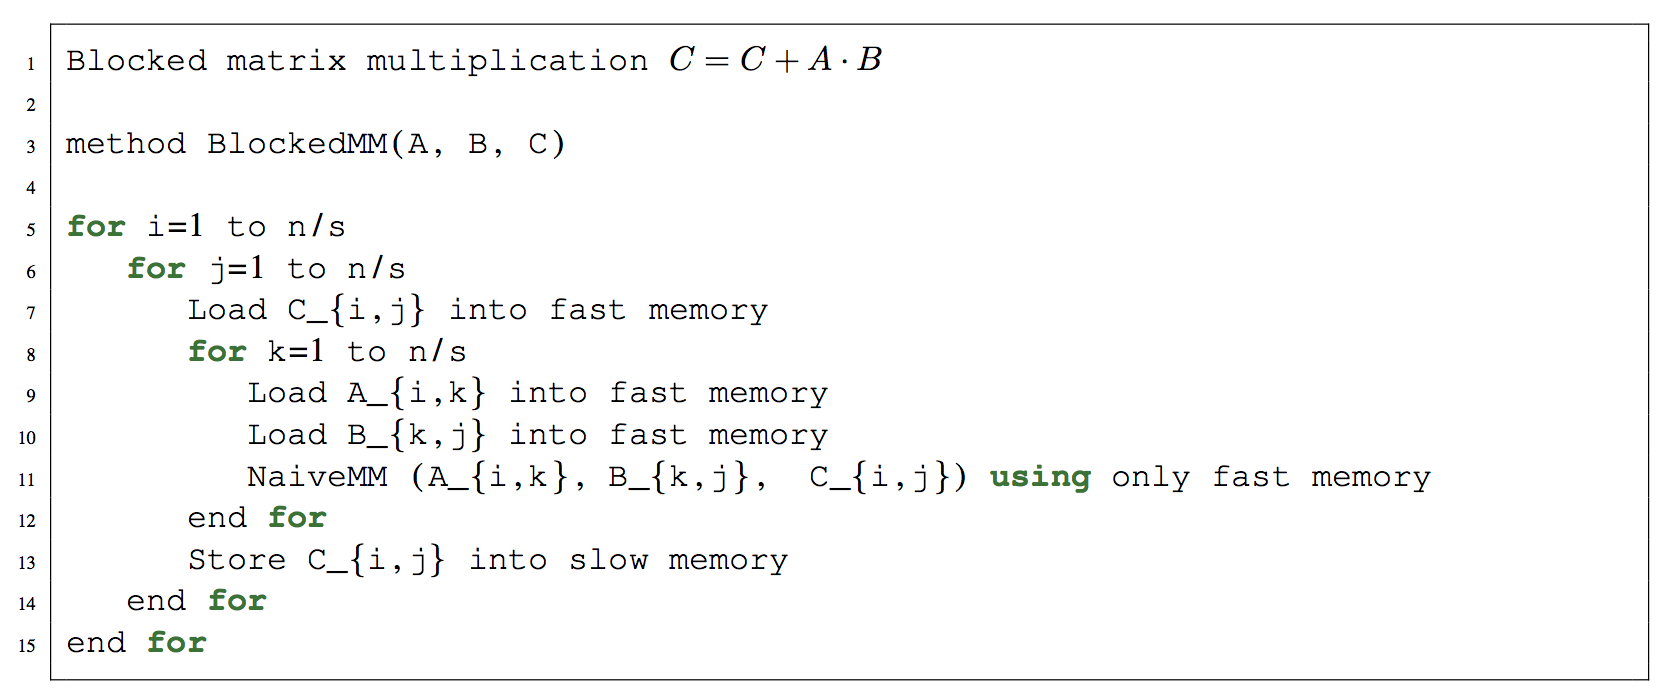
\includegraphics[width=\linewidth]{pseudocode}
                \caption{Pseudo-code provided on the motivation file}
                \label{pseudocode}
            \end{figure}

            \begin{figure}[H]
                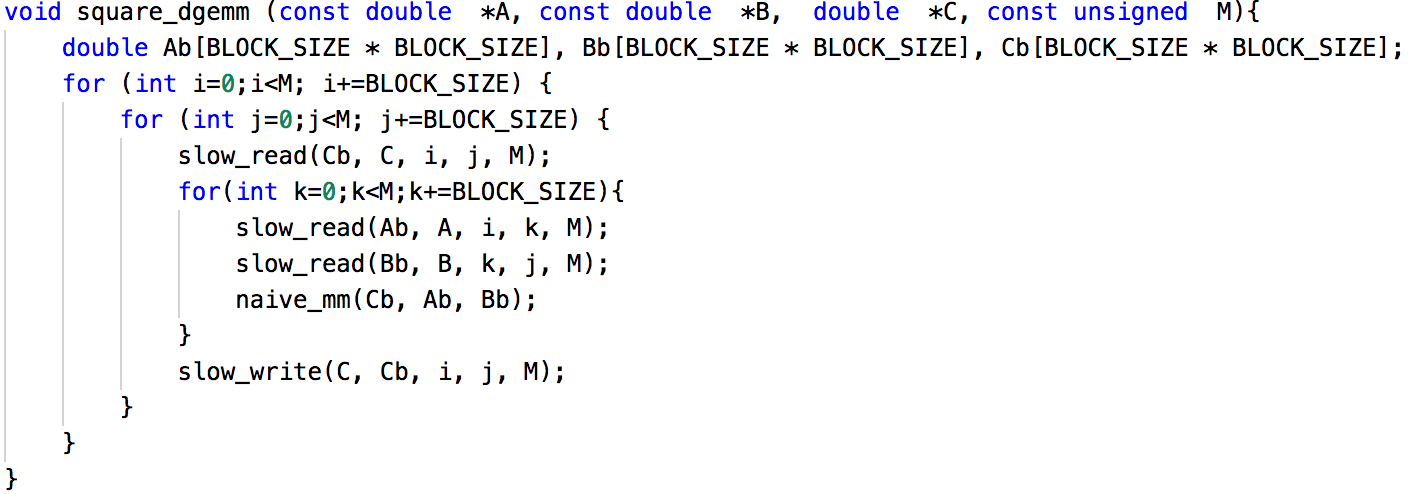
\includegraphics[width=\linewidth]{code}
                \caption{Function \textit{square\_dgemm} written}
                \label{code}
            \end{figure}

            The \textit{slow\_read} and \textit{slow\_write} functions can be seen in more detail in figures \ref{load} and \ref{write}.

            The \textit{slow\_read} function copies a submatrix of $BLOCK\_SIZE$ lines and columns from a matrix located in slow memory, arrays $A, B, C$, to the local arrays created, $Ab, Bb$ and $Cb$.

            In case the submatrix being copied is not interely inside the origin matrix, the copied matrix will be padded with zeroes.
            This is useful because it guarantees that the copied matrix has always the same dimensions: $BLOCK\_SIZE \times BLOCK\_SIZE$.

            \begin{figure}[H]
                \begin{minipage}{.48\textwidth}
                    \centering
                    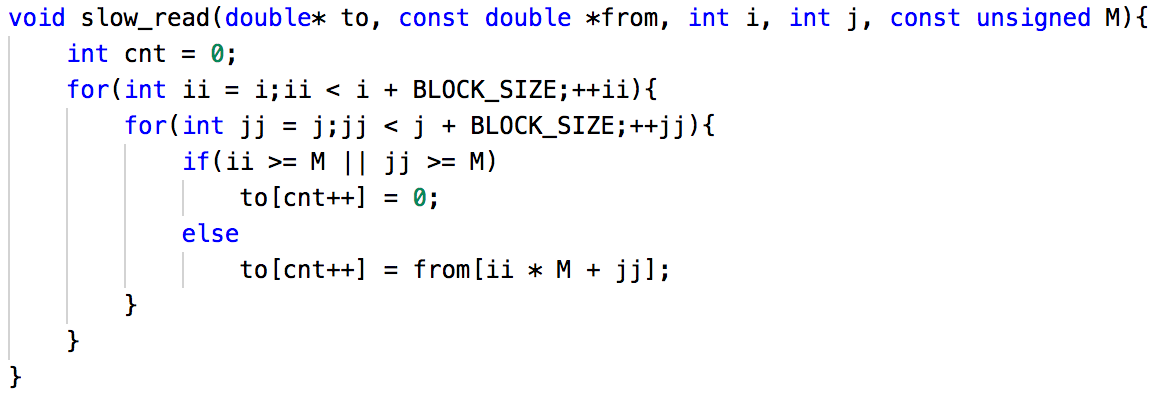
\includegraphics[width=\linewidth]{load}
                    \captionof{figure}{Load function}
                    \label{load}
                \end{minipage}%
                \hfill
                \begin{minipage}{.48\textwidth}
                    \centering
                    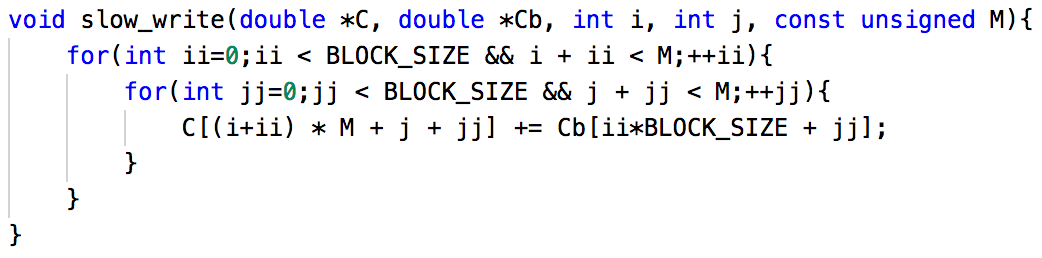
\includegraphics[width=\linewidth]{write}
                    \captionof{figure}{Store function}
                    \label{write}
                \end{minipage}
            \end{figure}

        The naive matrix multiplication only receives references to matrices on fast memory with dimensions $BLOCK\_SIZE \times BLOCK\_SIZE$ and does the classical algorithm for matrix multiplication.

            \begin{figure}[H]
                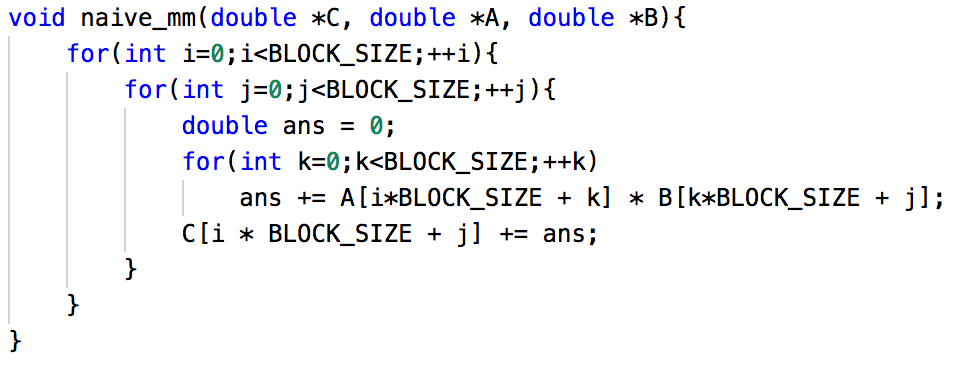
\includegraphics[width=\linewidth]{naive}
                \label{naive}
                \caption{Naive matrix multiplication}
            \end{figure}

            The best theoretical value for the block size is $\sqrt{M/3}$, being $M$ the size of the cache.

            Using only the cache L1 $M = 32kB$ (for icsmaster), that means that the optimal block size is $\sqrt{32kB/3} = 103B$ since every \textit{double} in C has $8B$, $103B \approx 37$ elements.
            Using the cache L2, with $M = 256kB$, the theoretical optimal block size is around 103 elements.

            In practice, though, one can notice that the block size that provides the best performance is $16$, as seen in the next question.


        \item 
            As previously stated the best performance was achieved by using a block size of $16$.

            Follows the graph plotted on my computer (Macbook Pro running macOS Sierra 10.12.6 with 2.5GHz Intel Core i7):

            \begin{figure}[H]
                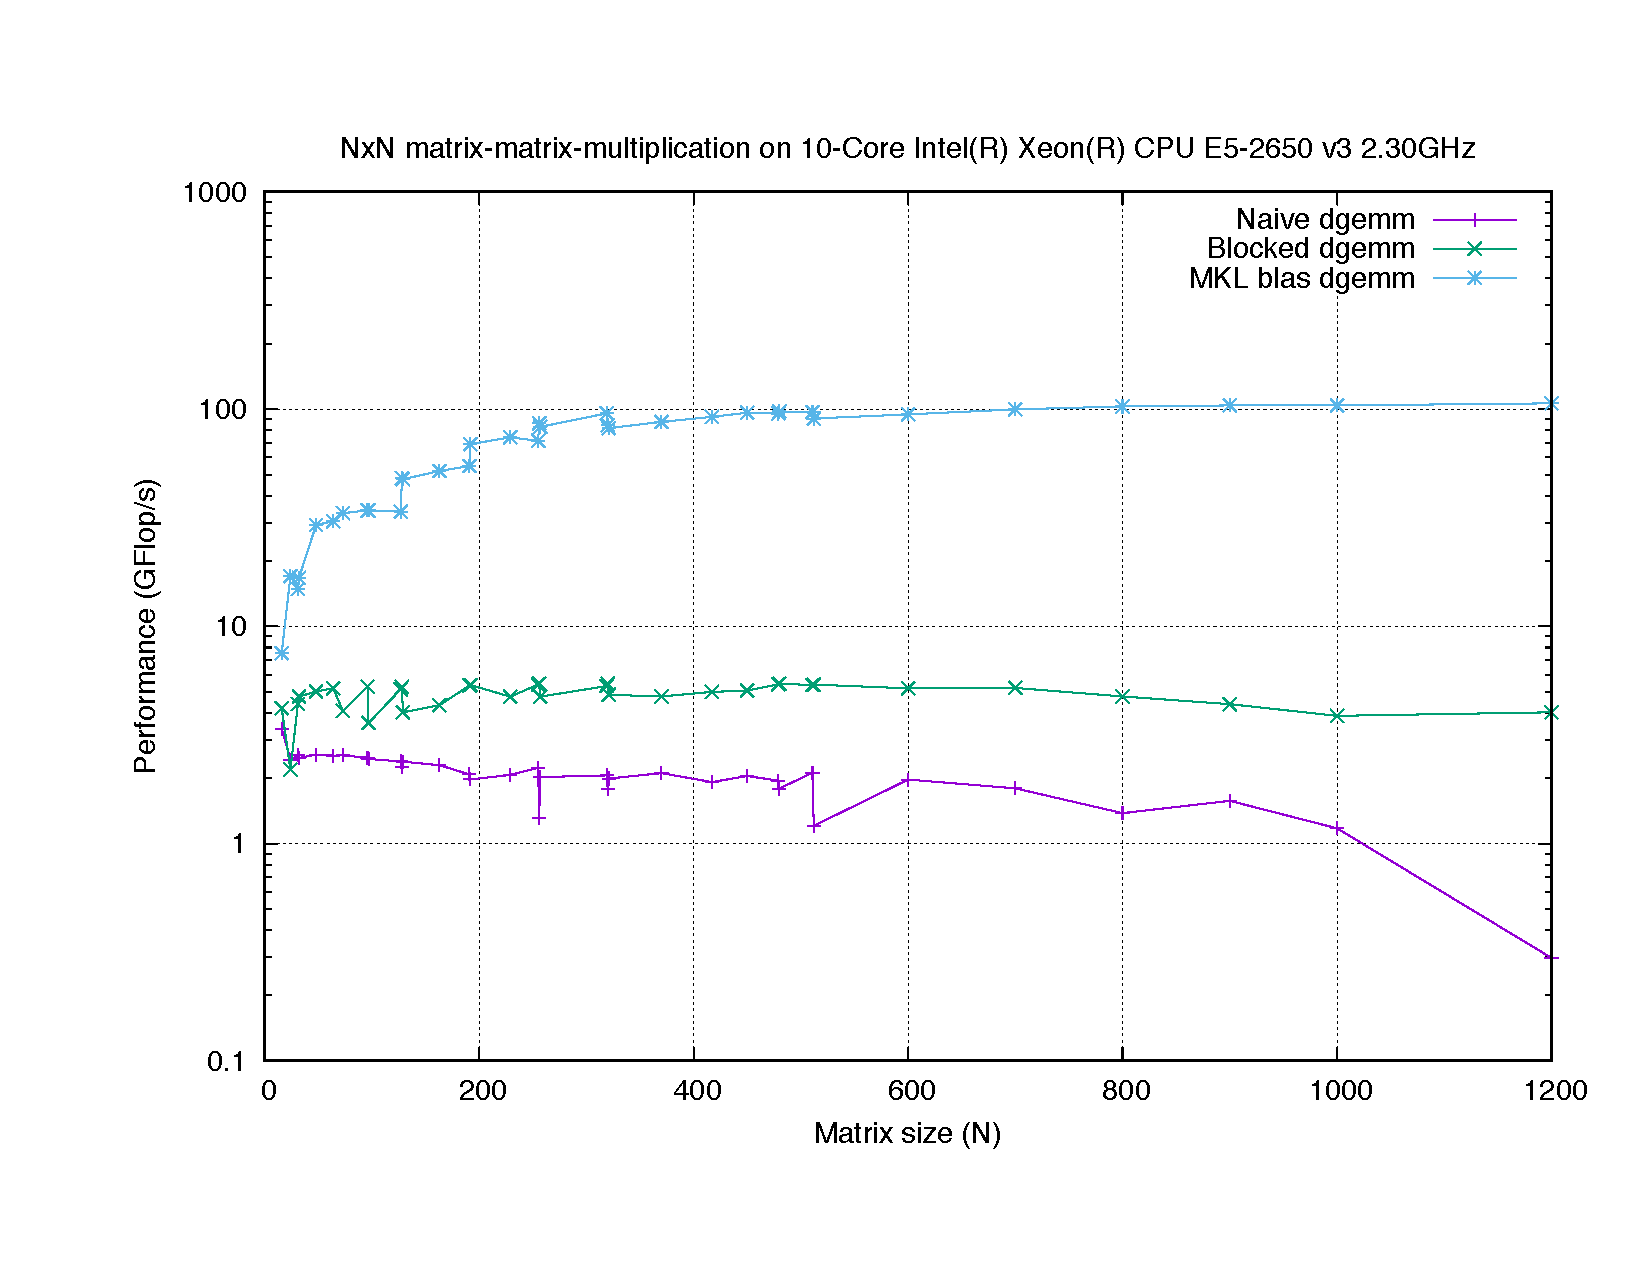
\includegraphics[width=.8\linewidth]{timing_mac}
                \caption{Graph for the experiment on Macbook Pro on macOS Sierra 10.12.6 on 2.5GHz Intel Core i7}
            \end{figure}

            \begin{figure}[H]
                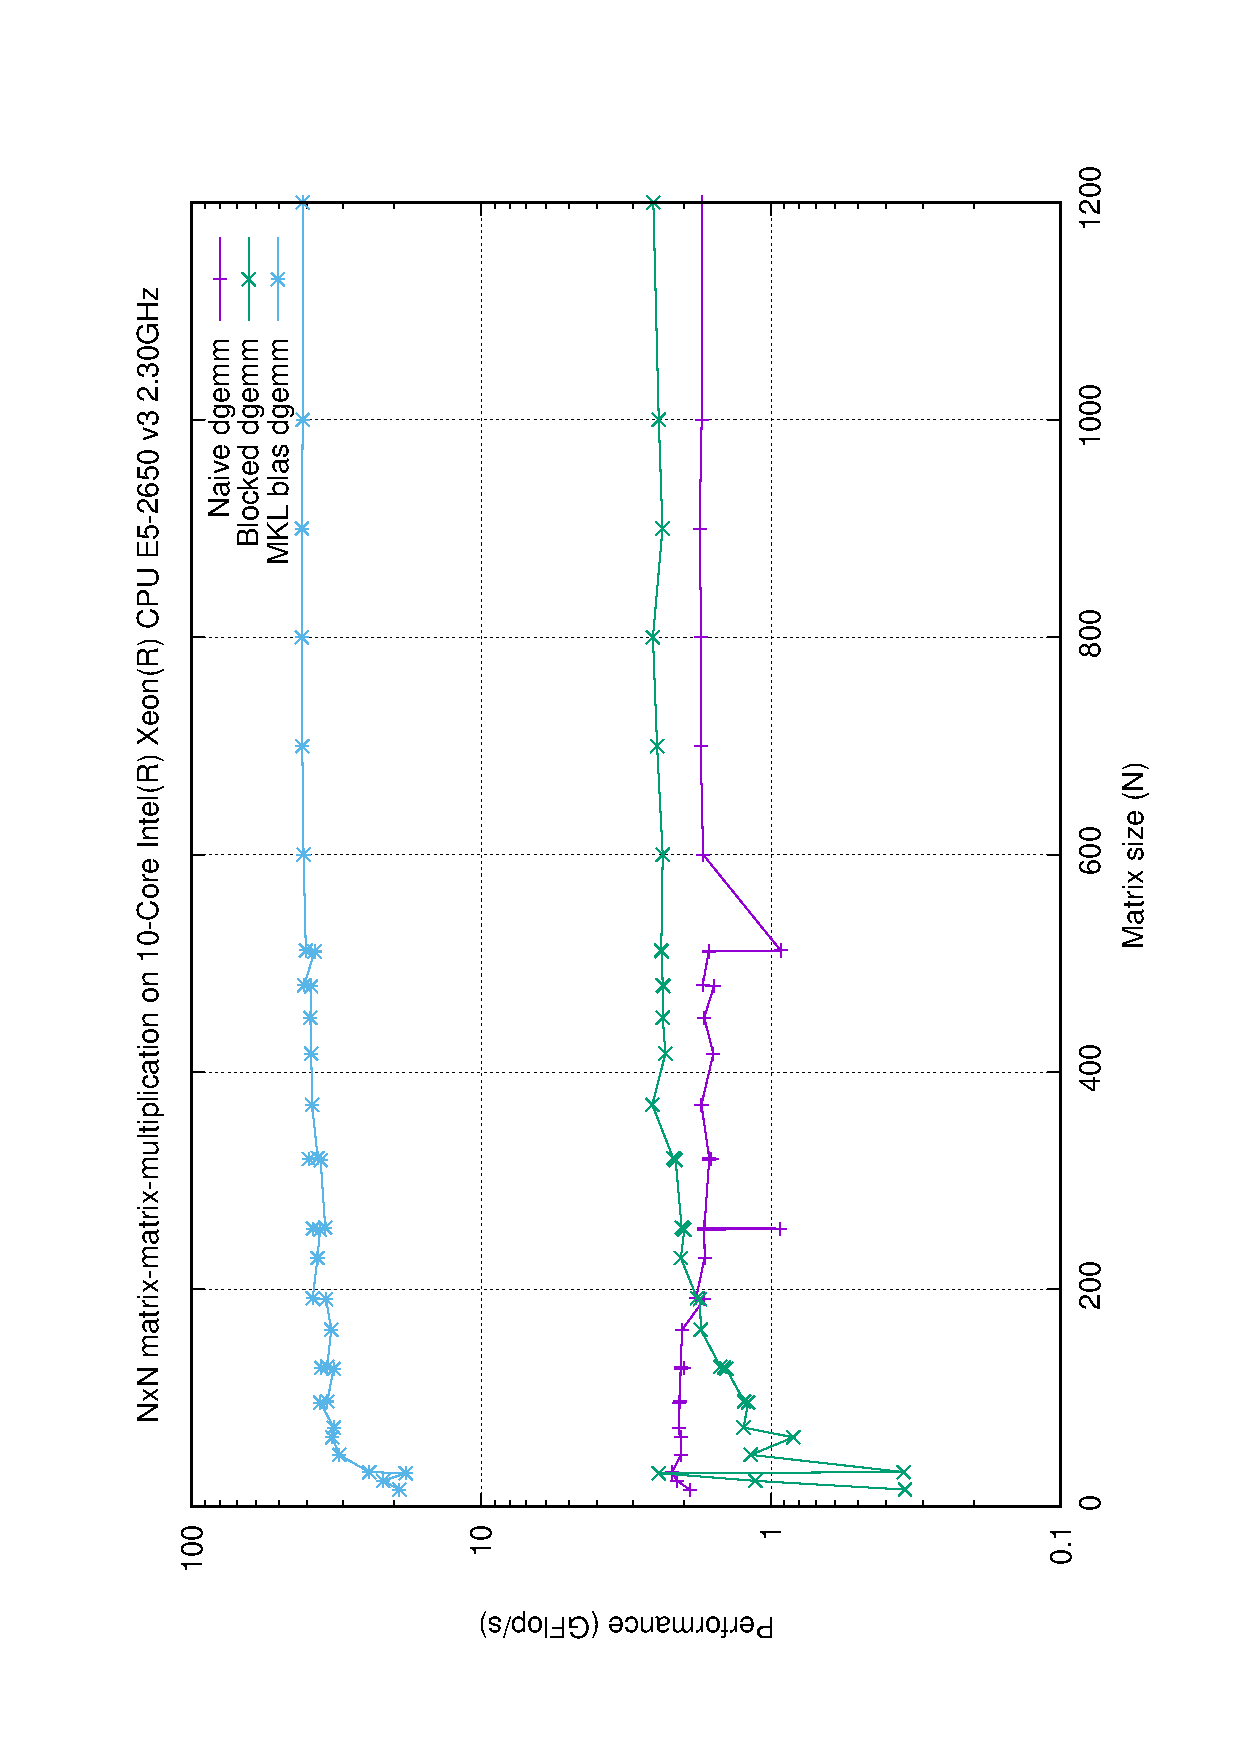
\includegraphics[width=.8\linewidth]{timing_icsmaster}
                \caption{Graph for the experiment on icsmaster}
            \end{figure}


            
        \item TODO: Explain the inhomogeneous behavior in performance curves.

        \item 
            There were two main differences in the performance between my machine and icsmaster.

            The first big difference is on the performance of "MKL blas dgemm".
            My machine reaches a plateau of about 100 GFlops/s, when the matrix size (N) is greater or equal to 300, whereas icsmaster reaches a plateau of about 30 GFLlops/s, when $N \geq 50$.

            This difference can be explained by analysing the difference in processors that my machine and icsmaster have.
            \sloppy Making a comparison in intel's website between my processor (Core i7-4870HQ) and icsmaster's processor (Xeon E5-2650) (the comparison can be seen in \href{https://ark.intel.com/content/www/us/en/ark/compare.html?productIds=83504,81705}{ark.intel.com/content/www/us/en/ark/compare.html?productIds=83504,81705}), one can see that my processor has better specifications, as shown in the following table:

            \begin{center}
                \begin{tabular}{| l || c | c |}
                        \hline
                    & \textbf{Macbook} & \textbf{icsmaster} \\
                    \hline
                    Processor base frequency & 2.50 GHz  & 2.30 GHz \\ 
                    \hline
                    Max Turbo frequency & 3.70 GHz & 3.00 GHz \\
                    \hline
                \end{tabular}
            \end{center}

            Intel's Math Kernel Library makes good use of this extra power present in my machine, running way more efficiently on my machine than on icsmaster. 


            The second big difference can be seen on the performance of the naive algorithm for $N \geq 700$. For this case my machine has a performance of 0.2 GFlops/s while icsmaster operates at about 1.1 GFlops/s. 

            This is due to the difference of cache L3 sizes between icsmaster and my machine.
            While icsmaster can hold up to 20MB in L3, my machine can only hold 6.3MB (information retrived by running \textit{sysctl hw.l3cachesize} on the terminal). 

            Three matrices of $N = 700$ occupy at least $N^2$ doubles, which can be translated to $3\times(700^2 \times 8 B) \approx 12$MB.
            This means that icsmaster can still hold these matrices on cache, but my machine has to fetch them from memory, explaining why my machine has a drop in performance for $N \geq 700$ whereas icsmaster can mantain a constant performance at about 1.1 GFlops/s.
            


        \item TODO: 

    \end{enumerate}

\end{document}
